\section{Evaluation}
\label{sec:evaluation}

Testbed settings..

\subsection{Microbenchmarks}

Use IPC-bench~\cite{ipc-bench} to benchmark Linux performance.

Linux socket vs \sys (intra-server socket, RDMA and libvma) performance comparison

Scenarios: connection setup and data transmission

Metrics: Latency, throughput

\begin{figure}[htpb]
	\centering
	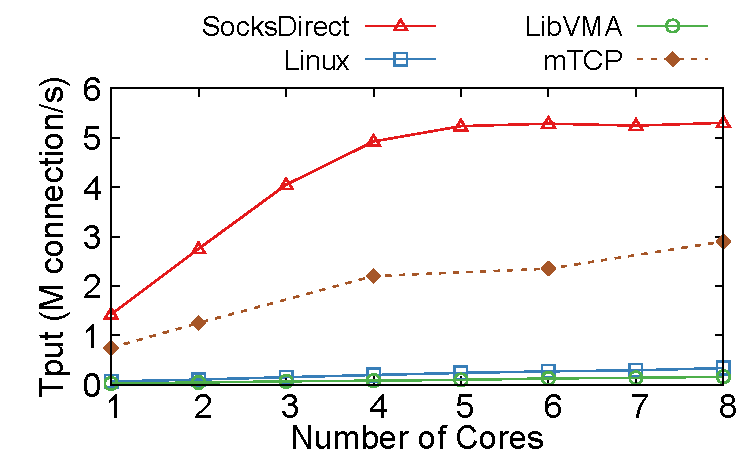
\includegraphics[width=\columnwidth]{eval/microbenchmark/conn-setup-tput.pdf}
	\caption{Throughput of the connection creation}
	\label{fig:eval-conn-setup-tput}
\end{figure}


\begin{figure}[htpb]
\centering                                                         
\subfloat[Intra-server]{                    
	%\begin{minipage}{0.4\textwidth}
	    \centering
	    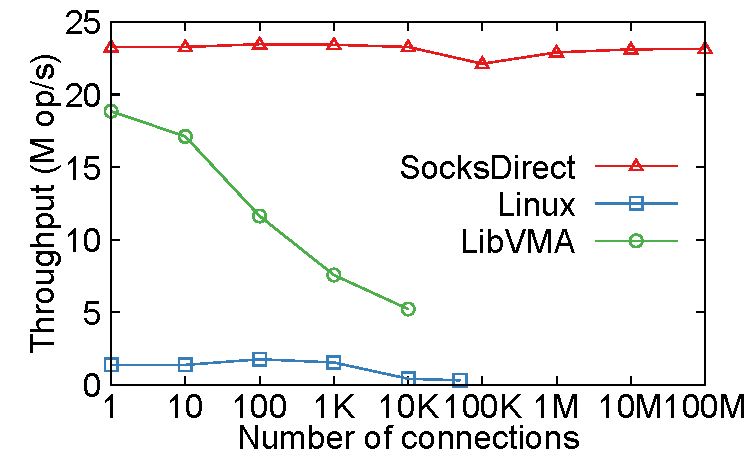
\includegraphics[width=\columnwidth]{eval/microbenchmark/connnum-ipc-tput.pdf}
	%\end{minipage}
	}

\subfloat[Inter-server]{
	%\begin{minipage}{0.4\textwidth}
		\centering                                                          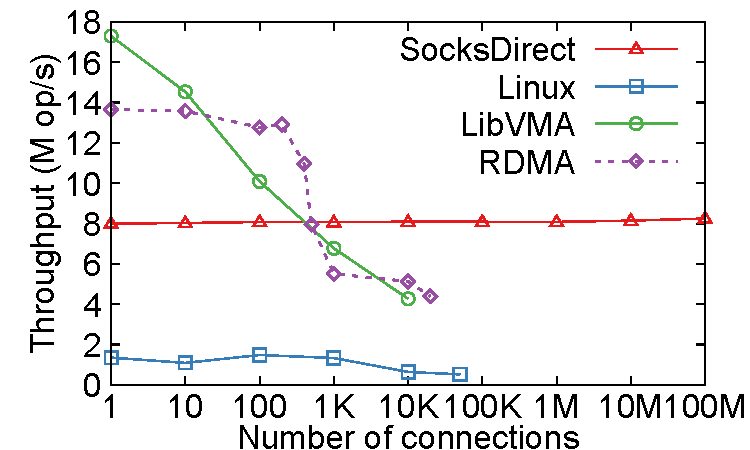
\includegraphics[width=\columnwidth]{eval/microbenchmark/connnum-network-tput.pdf}      
	%\end{minipage}
	}
	\caption{Throughput with different number of connections}
	\label{fig:eval-connnum-tput}                                           
\end{figure}

\begin{figure}[htpb]
	\centering
	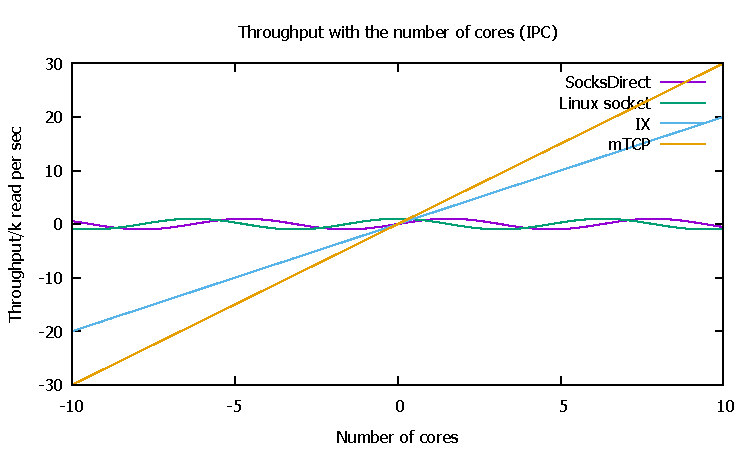
\includegraphics[width=\columnwidth]{eval/microbenchmark/cornum-IPC.pdf}
	\caption{Throughput with different number of cores for intra-server communication}
	\label{fig:eval-cornum-ipc}
\end{figure}

\begin{figure}[htpb]
	\centering                                                         
	\subfloat[Intra-server throughput]{                    
		%\begin{minipage}{0.4\textwidth}
			\centering
			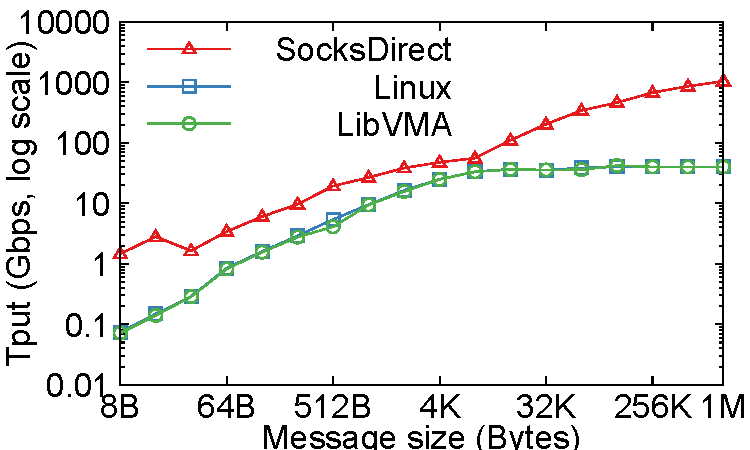
\includegraphics[width=\columnwidth]{eval/microbenchmark/msgsize-ipc-tput.pdf}
		%\end{minipage}
		}
	
	\subfloat[Inter-server throughput]{
		%\begin{minipage}{0.4\textwidth}
			\centering                                                          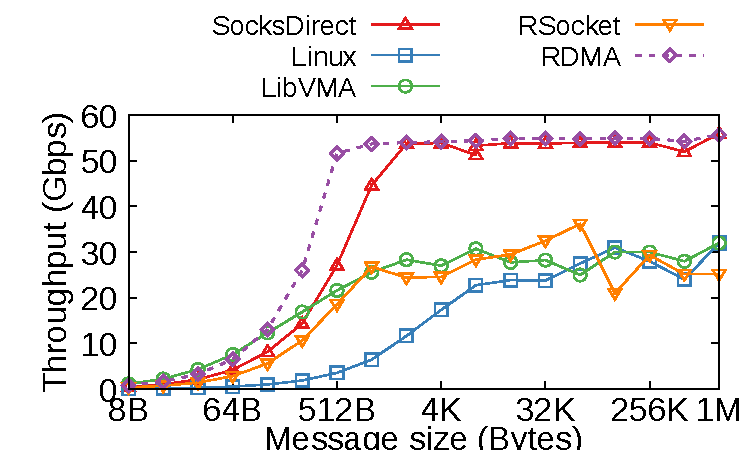
\includegraphics[width=\columnwidth]{eval/microbenchmark/msgsize-network-tput.pdf}      
		%\end{minipage}
		}

		\subfloat[Intra-server latency]{
		%\begin{minipage}{0.4\textwidth}
			\centering                                                          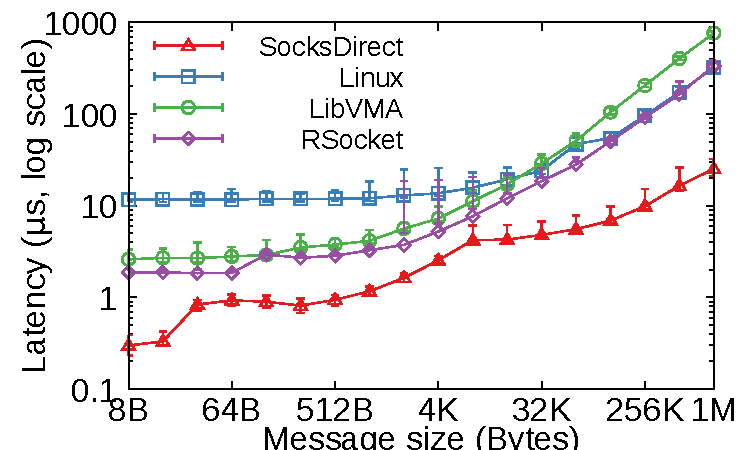
\includegraphics[width=\columnwidth]{eval/microbenchmark/msgsize-ipc-lat.pdf}      
		%\end{minipage}
		}

		\subfloat[Inter-server latency]{
		%\begin{minipage}{0.4\textwidth}
			\centering                                                          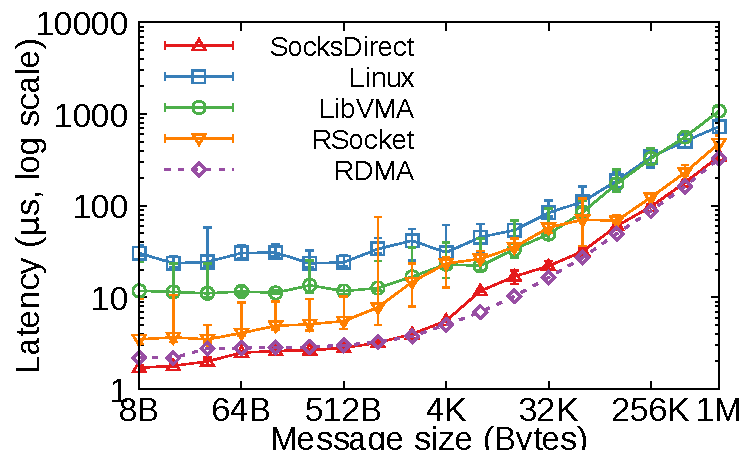
\includegraphics[width=\columnwidth]{eval/microbenchmark/msgsize-network-lat.pdf}      
		%\end{minipage}
		}
		\caption{Performance with different message size}
		\label{fig:eval-msgsize}                                           
\end{figure}





\subsection{Network Function}

Network functions~\cite{li2016clicknp}, ClickOS~\cite{martins2014clickos}

Scenarios: Firewall (no packet change), NAT (change a packet field), Tunnel endpoint (add/remove packet header, change length)

Metrics: Latency, throughput

\begin{figure}[htpb]
	\centering
	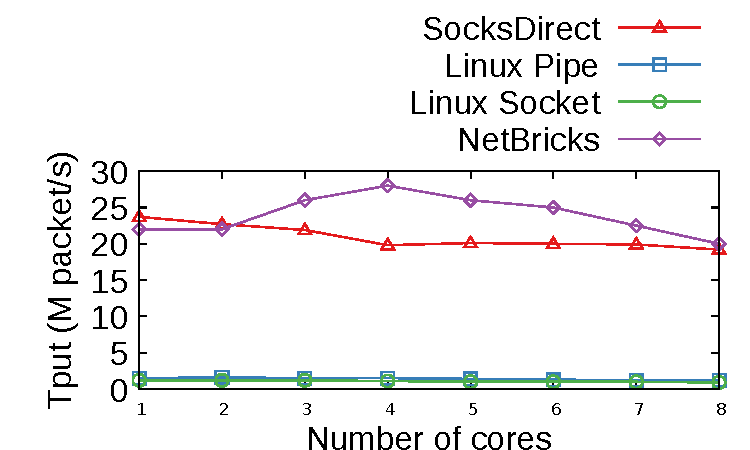
\includegraphics[width=\columnwidth]{eval/microbenchmark/nfv-tun-tput.pdf}
	\caption{Throughput of NFV tunnel}
	\label{fig:eval-tun-tput}
\end{figure}



\subsection{Web Application}

Nginx~\cite{nginx}, Nodejs~\cite{nodejs} and memcached~\cite{memcached}

\begin{itemize}
	\item Many short-lived connections. Nginx $\rightarrow$ Nodejs, Nodejs access memcached once.
	\item Each connection, backend interact extensively. (Nodejs access memcached multiple round trips.)
	\item Long connection to download a large in-memory file. (test zero copy)
\end{itemize}

\begin{figure}[htpb]
	\centering                                                         
	\subfloat[Short-lived connections]{                    
		%\begin{minipage}{0.4\textwidth}
			\centering
			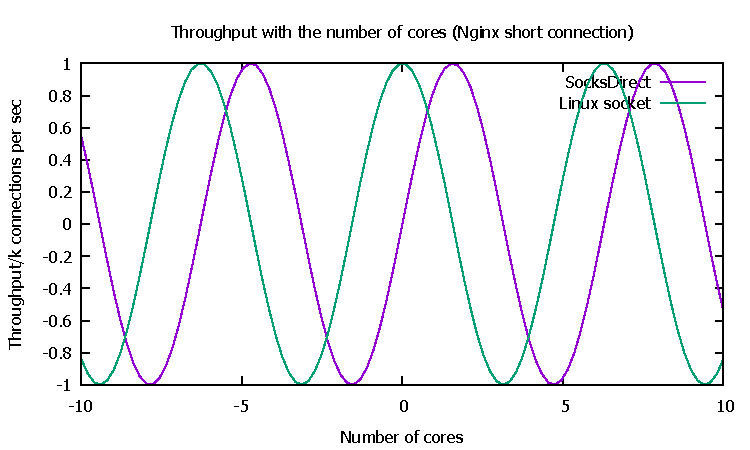
\includegraphics[width=\columnwidth]{eval/microbenchmark/nginx-short-tput.pdf}
		%\end{minipage}
		}
	
	\subfloat[Multiple round-trip short-lived connections]{
		%\begin{minipage}{0.4\textwidth}
			\centering                                                          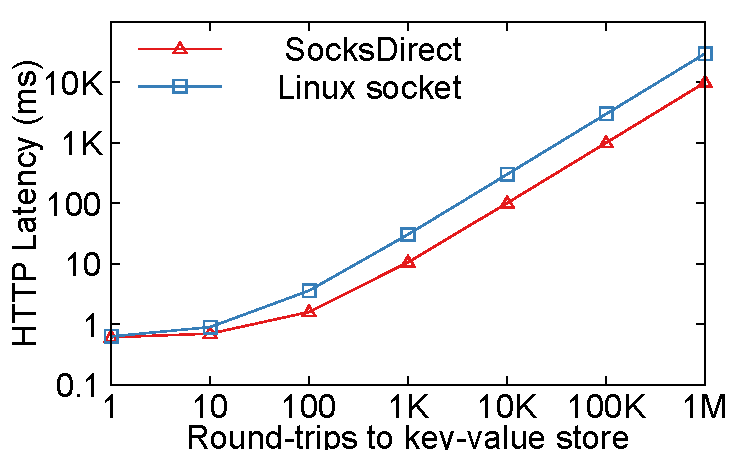
\includegraphics[width=\columnwidth]{eval/microbenchmark/nginx-multiround-tput.pdf}      
		%\end{minipage}
		}

		\subfloat[Long-lived connections]{
		%\begin{minipage}{0.4\textwidth}
			\centering                                                          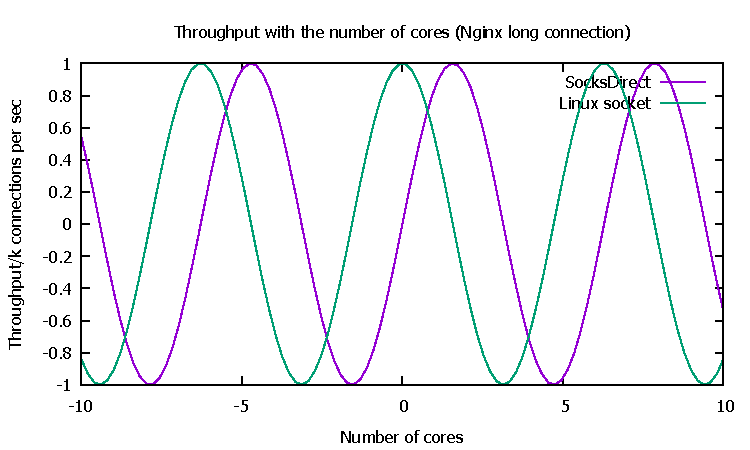
\includegraphics[width=\columnwidth]{eval/microbenchmark/nginx-long-tput.pdf}      
		%\end{minipage}
		}
		
		\caption{Throughput of nginx}
		\label{fig:eval-nginx-tput}                                           
\end{figure}


%\subsection{Real-time Stream Processing}

%Apache Flink~\cite{carbone2015apache} (need to turn off durability on disk)

%Scenario: Word Count (distributed system with one source, two mappers and one reducer)

%Metrics: Latency, throughput

%\subsection{Machine Learning}

%Tensorflow~\cite{abadi2016tensorflow}

%Scenario: (Distributed Tensorflow) Parameter server and worker on a same server.

%Metrics: Time per iteration